\subsubsection{Pascalsches Dreieck}
\label{subsubsec:fundamentals_pascals_triangle}

Die Binomialkoeffizienten können alternativ ohne Fakultäten aus dem
Pascalschen Dreieck abgelesen werden. Seine Konstruktion folgt zwei einfachen
Regeln:
\begin{itemize}
  \item Jede Zeile beginnt und endet mit einer $1$.
  \item Jede innere Zahl ist die Summe der beiden schräg darüberstehenden
    Zahlen.
\end{itemize}

\begingroup
\newcommand{\PascalTriangleFigure}{%
\begin{center}
\begin{tikzpicture}[
    x=1.15cm,
    y=0.8cm,
    every node/.style={font=\small,minimum width=6mm,minimum height=6mm}
  ]
  % Für festes k verlaufen die Einträge schräg von rechts oben nach links unten.
  \foreach \k in {0,...,5} {
    \draw[THMBlue!70,dashed,thick,->]
      ({0.5*\k},{-\k}) -- ({\k-3},-6);
    \node[THMBlue,fill=white,inner sep=1pt] at ({\k-3},-6.35) {$k=\k$};
  }

  \node[anchor=east,text=black!55] at (-3.4,0) {$n=0$};
  \node[fill=white] at (0,0) {$1$};

  \node[anchor=east,text=black!55] at (-3.4,-1) {$n=1$};
  \node[fill=white] at (-0.5,-1) {$1$};
  \node[fill=white] at (0.5,-1) {$1$};

  \node[anchor=east,text=black!55] at (-3.4,-2) {$n=2$};
  \node[fill=white] at (-1,-2) {$1$};
  \node[fill=white] at (0,-2) {$2$};
  \node[fill=white] at (1,-2) {$1$};

  \node[anchor=east,text=black!55] at (-3.4,-3) {$n=3$};
  \node[fill=white] at (-1.5,-3) {$1$};
  \node[fill=white] at (-0.5,-3) {$3$};
  \node[
    fill=white,
    draw=olive!85!black,
    very thick,
    rounded corners=2pt,
    inner sep=2pt
  ] (exampleCoefficient) at (0.5,-3) {$3$};
  \node[fill=white] at (1.5,-3) {$1$};

  \node[anchor=east,text=black!55] at (-3.4,-4) {$n=4$};
  \node[fill=white] at (-2,-4) {$1$};
  \node[fill=white] at (-1,-4) {$4$};
  \node[fill=white] at (0,-4) {$6$};
  \node[fill=white] at (1,-4) {$4$};
  \node[fill=white] at (2,-4) {$1$};

  \node[anchor=east,text=black!55] at (-3.4,-5) {$n=5$};
  \node[fill=white] at (-2.5,-5) {$1$};
  \node[fill=white] at (-1.5,-5) {$5$};
  \node[fill=white] at (-0.5,-5) {$10$};
  \node[fill=white] at (0.5,-5) {$10$};
  \node[fill=white] at (1.5,-5) {$5$};
  \node[fill=white] at (2.5,-5) {$1$};

  \node[
    anchor=west,
    font=\normalsize,
    fill=white,
    text=olive!85!black,
    inner sep=2pt
  ] (exampleCoefficientLabel) at (2.8,-2.45)
    {$\binom{3}{2}=3$};
  \draw[olive!85!black,very thick]
    (exampleCoefficient.north) -- ++(0,0.18) -- (exampleCoefficientLabel.west);

\end{tikzpicture}
\end{center}
}
\newcommand{\PascalTriangleGrid}{%
  \par\medskip\noindent
  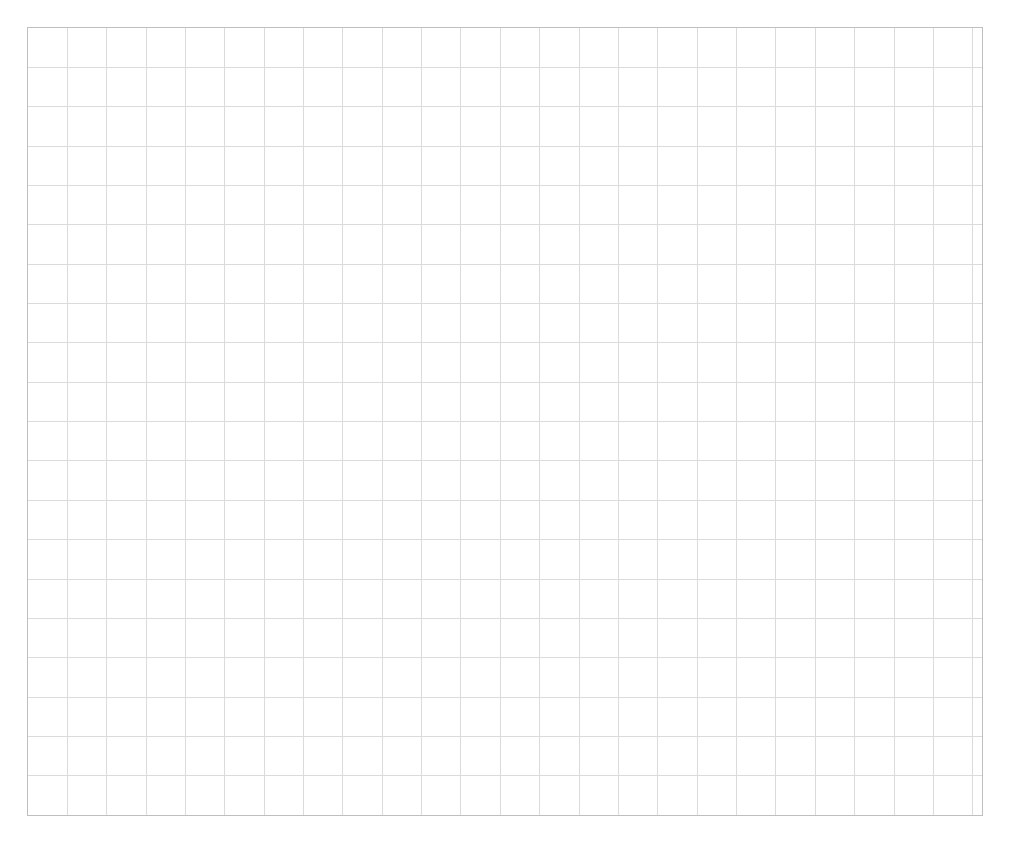
\begin{tikzpicture}[baseline=(current bounding box.north)]
    \path[use as bounding box] (0,0) rectangle (\linewidth,-10cm);
    \draw[step=5mm,black!14,line width=0.2pt]
      (0,0) grid (\linewidth,-10cm);
    \draw[black!25,line width=0.3pt]
      (0,0) rectangle (\linewidth,-10cm);
  \end{tikzpicture}%
  \par\medskip
}
\IfClozeTF{\PascalTriangleGrid}{\PascalTriangleFigure}
\endgroup

\noindent\begin{minipage}{\linewidth}
\begin{KeyPointBox}{Binomialkoeffizienten im Pascalschen Dreieck}%
  {fundamentals_pascal_triangle_binomial_coefficients}
  Im Pascalschen Dreieck stehen alle Binomialkoeffizienten $\binom{n}{k}$.
  \begin{center}
    \begin{tikzpicture}
      \node[inner sep=0pt,font=\Large] (coefficient)
        {$\displaystyle\binom{n}{k}$};

      \node[anchor=west,font=\normalsize] (rowLabel)
        at (2.2cm,0.6cm) {Zeile im Dreieck};
      \node[anchor=west,font=\normalsize] (columnLabel)
        at (2.2cm,-0.6cm) {Spalte im Dreieck};

      \draw[black,thick,-{Stealth[length=2mm]}]
        ([xshift=0.6mm,yshift=4.1mm]coefficient.east)
        -- ([xshift=-1.5mm]rowLabel.west);
      \draw[black,thick,-{Stealth[length=2mm]}]
        ([xshift=0.6mm,yshift=-4.1mm]coefficient.east)
        -- ([xshift=-1.5mm]columnLabel.west);
    \end{tikzpicture}
  \end{center}
  Damit lassen sich die Koeffizienten einer binomischen Formel direkt aus der
  Zeile $n$ ablesen.
\end{KeyPointBox}

\begin{ExampleBox}{Binomische Formel für $n=5$}%
  {fundamentals_pascal_triangle_binomial_formula_n_five}
  Die Koeffizienten der binomischen Formel liefert uns direkt die Zeile $n=5$
  im Pascalschen Dreieck:
  \begin{center}
    \begin{tikzpicture}
      \matrix (coefficientMap) [
        matrix of math nodes,
        nodes={font=\normalsize,inner sep=1pt,anchor=base},
        column sep=1.5pt,
        row sep=1.5mm
      ] {
        {}
          & |[text=black!55]| \displaystyle\binom{5}{0} & {} & {}
          & |[text=black!55]| \displaystyle\binom{5}{1} & {} & {}
          & |[text=black!55]| \displaystyle\binom{5}{2} & {} & {}
          & |[text=black!55]| \displaystyle\binom{5}{3} & {} & {}
          & |[text=black!55]| \displaystyle\binom{5}{4} & {} & {}
          & |[text=black!55]| \displaystyle\binom{5}{5} & {} \\
        {}
          & |[text=black!55]| \rotatebox[origin=c]{90}{$=$} & {} & {}
          & |[text=black!55]| \rotatebox[origin=c]{90}{$=$} & {} & {}
          & |[text=black!55]| \rotatebox[origin=c]{90}{$=$} & {} & {}
          & |[text=black!55]| \rotatebox[origin=c]{90}{$=$} & {} & {}
          & |[text=black!55]| \rotatebox[origin=c]{90}{$=$} & {} & {}
          & |[text=black!55]| \rotatebox[origin=c]{90}{$=$} & {} \\
        |[text=black!55]| n=5:
          & |[draw=THMBlue,very thick,rounded corners=2pt,minimum width=8mm,minimum height=8mm]| \Cloze{7mm}{1}
          & {} & {}
          & |[draw=THMBlue,very thick,rounded corners=2pt,minimum width=8mm,minimum height=8mm]| \Cloze{7mm}{5}
          & {} & {}
          & |[draw=THMBlue,very thick,rounded corners=2pt,minimum width=8mm,minimum height=8mm]| \Cloze{7mm}{10}
          & {} & {}
          & |[draw=THMBlue,very thick,rounded corners=2pt,minimum width=8mm,minimum height=8mm]| \Cloze{7mm}{10}
          & {} & {}
          & |[draw=THMBlue,very thick,rounded corners=2pt,minimum width=8mm,minimum height=8mm]| \Cloze{7mm}{5}
          & {} & {}
          & |[draw=THMBlue,very thick,rounded corners=2pt,minimum width=8mm,minimum height=8mm]| \Cloze{7mm}{1}
          & {} \\[5mm]
        (a+b)^5=
          & \Cloze{7mm}{\textcolor{THMBlue}{1}} & a^5 & +
          & \Cloze{7mm}{\textcolor{THMBlue}{5}} & a^4b & +
          & \Cloze{7mm}{\textcolor{THMBlue}{10}} & a^3b^2 & +
          & \Cloze{7mm}{\textcolor{THMBlue}{10}} & a^2b^3 & +
          & \Cloze{7mm}{\textcolor{THMBlue}{5}} & ab^4 & +
          & \Cloze{7mm}{\textcolor{THMBlue}{1}} & b^5 \\
      };

      \foreach \column in {2,5,8,11,14,17} {
        \draw[THMBlue!75,thick,-{Stealth[length=2mm]}]
          (coefficientMap-3-\column.south)
          -- (coefficientMap-4-\column.north);
      }
    \end{tikzpicture}
  \end{center}
\end{ExampleBox}
\end{minipage}

\begin{RemarkBox}[
  remark title=\Lang{Eigenschaften der Binomialkoeffizienten}{Properties of binomial coefficients},
  breakable=false
]
  Für die Binomialkoeffizienten gelten folgende Eigenschaften:
  \begin{itemize}
    \item In jeder Zeile sind die beiden Randwerte gleich $1$ und die unmittelbar danebenliegenden Werte gleich $n$
      \begin{center}
        \IfClozeTF{%
          
\begin{tikzpicture}[baseline=(current bounding box.center)]
            \draw[step=5mm,black!14,line width=0.2pt]
              (0,0) grid (40mm,10mm);
            \draw[black!25,line width=0.3pt]
              (0,0) rectangle (40mm,10mm);
          \end{tikzpicture}
          \qquad und \qquad
          
\begin{tikzpicture}[baseline=(current bounding box.center)]
            \draw[step=5mm,black!14,line width=0.2pt]
              (0,0) grid (40mm,10mm);
            \draw[black!25,line width=0.3pt]
              (0,0) rectangle (40mm,10mm);
          \end{tikzpicture}%
        }{%
          $\displaystyle
            \binom{n}{0}=1=\binom{n}{n}
            \qquad \text{und} \qquad
            \binom{n}{1}=n=\binom{n}{n-1}.$%
        }
      \end{center}
    \item Das Pascalsche Dreieck ist bezüglich seiner Mitte symmetrisch:
      \begin{ClozeArea}[14]{2}
        \centering
        $\displaystyle
          \binom{n}{k}=\binom{n}{n-k}.$
      \end{ClozeArea}
      Anschaulich bedeutet dies, dass sich jede Zeile wie ein
      \Cloze{5cm}{Palindrom} in der Sprachwissenschaft liest.
  \end{itemize}
\end{RemarkBox}

